\documentclass[tikz,border=10pt]{standalone}
\begin{document}
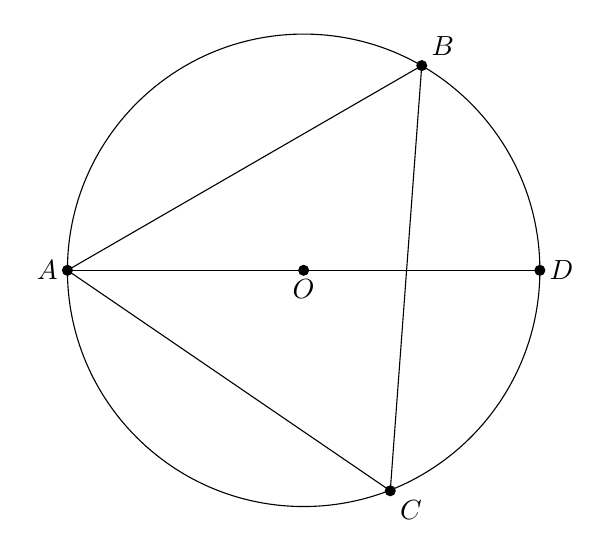
\begin{tikzpicture}[scale=1]

\coordinate (O) at (0,0);
\coordinate (A) at (-3,0);
\coordinate (D) at (3,0);
\coordinate (B) at (1.5,2.6);
\coordinate (C) at (1.1,-2.8);

\draw (O) circle[radius=3];
\draw (A) -- (D);
\draw (A) -- (B);
\draw (A) -- (C);
\draw (B) -- (C);

\fill (A) circle (2pt);
\fill (B) circle (2pt);
\fill (C) circle (2pt);
\fill (D) circle (2pt);
\fill (O) circle (2pt);

\node[left] at (A) {$A$};
\node[above right] at (B) {$B$};
\node[below right] at (C) {$C$};
\node[right] at (D) {$D$};
\node[below] at (O) {$O$};

\end{tikzpicture}
\end{document}
